\documentclass{report}
\usepackage[left=3cm]{geometry}
\usepackage{verbatim}
\usepackage{graphicx}
\usepackage{tabularx}
\setlength{\extrarowheight}{5pt}

\begin{document}
\title{Poker Project}
\author{MINGKUN YANG ID:900506-T073\\
minyan09@student.hh.se\\
XIAO TAN ID:870426-0887\\
xiatan10@student.hh.se\\
}
\maketitle 

\section{Background}
There are two places the agent needs to make some decisions. Firstly, the agent has the freedom to discard any number of cards after the first 
betting round. Secondly, the agent has a few options in the betting round(first and second).

\section{Discussion}
\subsection{Discard cards}
First decision is easier to make. The only input the current hand, which contains five cards. We could define one space such that each state in this 
space represents one particular hand. States are connected by edges and each edge has one associated cost, which is the number of different cards in 
two hands. Utility is defined with categories according to the rules of this game. Each category has the utility: $u_i = 1/p_i$, where $p_i$ is the 
probability of this category appears in all cases.

Apparently, this graph is fully connected and $0 \le Cost \le 5$. The goal is to find which cards should be discarded. The evaluation function is 
based on which category this hand is. In other words, the expected utility will be maximum after discards certain cards, and this function return this
information to us.

The implementation in this case is to iterate all kinds of possibilities and calculate the mean value. There are five cards in one hand, and every 
card can be discarded, which means that there are $2^5$ possibilities and this function calculate the utility for the new hand and average the sum so 
that we know what the expect utility is of this possibility. Eventually, we find the maximum by comparing all of them and return the corresponding 
strategy.

Intuitively, the expected utility of discarding all the cards will always be smaller than some cases of discarding two or three cards, because it is 
always better to work on the basis of something instead of starting from scratch. Then, one interesting question arises: what is the smallest number 
of cards can be discarded, if it exists.
\[ \exists n \forall x<n, u_n < Max(u_x) \]
,where $u_n$ is the utility of any new hand after discarding $n$ cards. In other words, the question is the above assertion is right and we need to 
find the smallest $n$. It's easy to show that the assertion is true, for we've found one number, which is five. How about four? I don't how to prove 
this without resort to enumeration.

Since it's not necessary to calculate the cases for $n=4, 5$, this function can respond within a short time.
\subsection{Betting}
This problem is much harder than previous one, for the input value contains the current hand, other players' bet and other players' strategy. The 
corresponding Bayesian network is shown below. If the environment is fully observable for our agent, then it's trivial to make the decision, and the 
Bayesian network is totally different as well. In this game, ``Opponent's Hand'' is not accessible and the agent needs to infer it from ``Opponent's 
Bet''. Usually, one player would bet more if he or she has a good hand. There is one exception to this: bluffing.
\begin{figure}[t]
	\begin{center}
		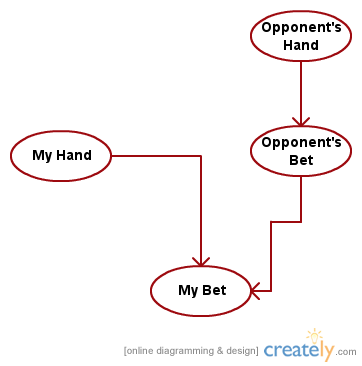
\includegraphics[scale=0.5]{PokerBayesianNetwork.png}
		\caption{Poker Bayesian Network}
	\end{center}
\end{figure}

There are two betting rounds totally, and the only difference is the expected utility for the opponents varies. In the first betting round, the 
expected utility is 9.
\[ u = \sum_{i=1}^{9} P_i U_i \]
.where $U_i$ is defined to be $1/P_i$ and there are nine categories totally.

Before the second betting round, we know how many cards each opponent has discarded, and we can calculate the expected utility after discarding 
certain number of cards($n$). Similar to previous dilemma, I could not come up with any solution except iterating all the possibilities and get the 
mean value.

So far we have the utility for our hand and the expected utility of opponent's hand, and we are able to do the betting. Based on ``Opponent's Bet'', 
the agent should adjust its belief. However, what's the optimal adjust is still too complex to be answered.

The following is the guideline the agent is supposed to use. A couple of functions and variables exist in this flow chart and need some explanation. 

``Number of allins'' is used to infer how many players have already taken ``allin'' action. Of course, the agent needs to listen to the server 
carefully, for the server will broadcast the action other players have taken. 

``Is he bluffing'' is used to infer whether this action is his or her bluffing. The rationale is that once the frequency of ``allin'' from this 
specific palyer has reach the threshold, the agent should assume he or she is bluffing. The exact value for threshold is open to debate.

``utility'' refers to the utility of the current hand, and ``expectedUtility'' is the expected utility following the optimal stragegy of discarding 
some cards. ``expectedOpponentUtility'' and ``newExpectedOpponentUtility'' mean the same.

\begin{figure}[t]
	\begin{center}
		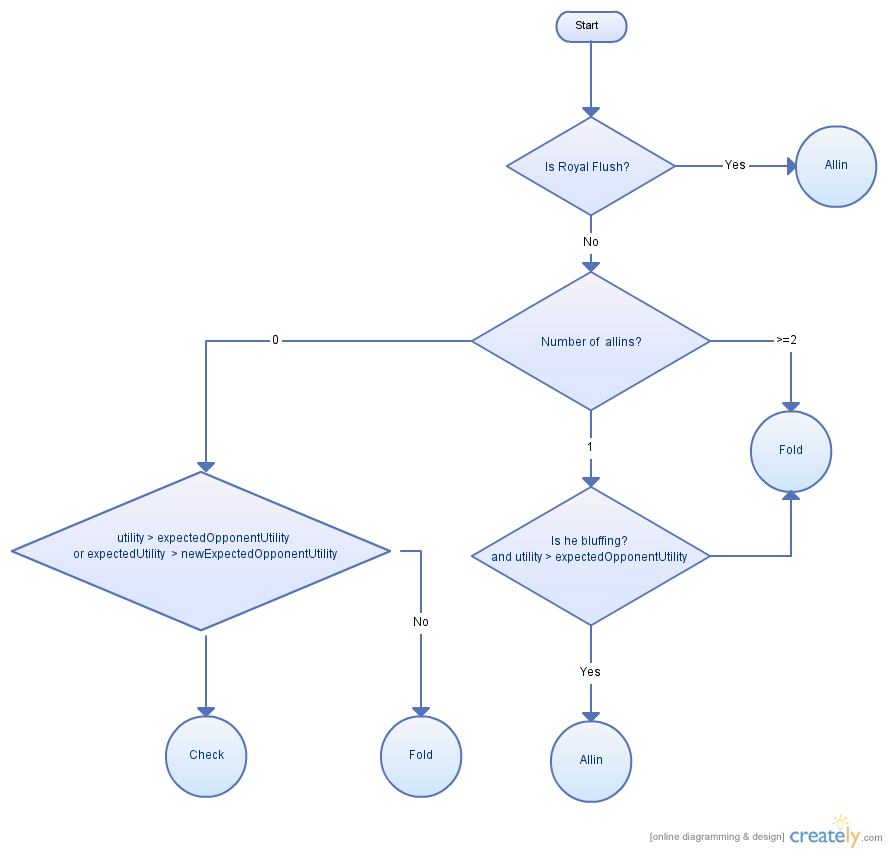
\includegraphics[scale=0.4]{PokerFlowChart.png}
		\caption{Poker Flow Chart}
	\end{center}
\end{figure}

\section{Limitation}
A lot of parameters need to be tuned in order to get good performance. Ideally, all these parameters can be optimized theoretically. Unfortunately, I 
don't know how to achieve it.

Inspect the flow chart of decision, and we can see that the agent will never choose ``raise'' action, which probably implies that this agent is not 
the optimal agent, for sometimes the agent might just raise a small amount of money gradually, which lures the opponents to ``check''. Eventually, 
they will have to ``check'' all the ``raise'' or just fold. Using this, we can avoid scare opponents away by just ``allin''.

\section{Conclusion}
The above discussion provides one clear and high level view for the whole problem, but the core difficult has been solved: the optimal adjustment 
according to ``Opponent's Bet''. Intuitively, there is supposed to be one optimal solution, which enable this agent to beat all other agents in the 
long run and is the first to do that.
\end{document}
